\documentclass[10pt,twocolumn,letterpaper]{article}

\usepackage[review]{cvpr}
\usepackage{graphicx}
\usepackage{amsmath,amssymb}
\usepackage{booktabs}
\usepackage{multirow}
\usepackage{caption}
\usepackage{xcolor}
\usepackage[colorlinks=true,allcolors=blue]{hyperref}
\usepackage[capitalize]{cleveref}

\def\cvprPaperID{****}
\def\confName{CVPR}
\def\confYear{2026}

\title{FTW-Planet: Pairing Fields of The World with 3\,m PlanetScope Imagery for Field-Boundary Segmentation}

\author{Anonymous EarthVision submission\\
Paper ID \cvprPaperID}

\begin{document}
\twocolumn[{%
\renewcommand\twocolumn[1][]{#1}%
\maketitle
\begin{center}
    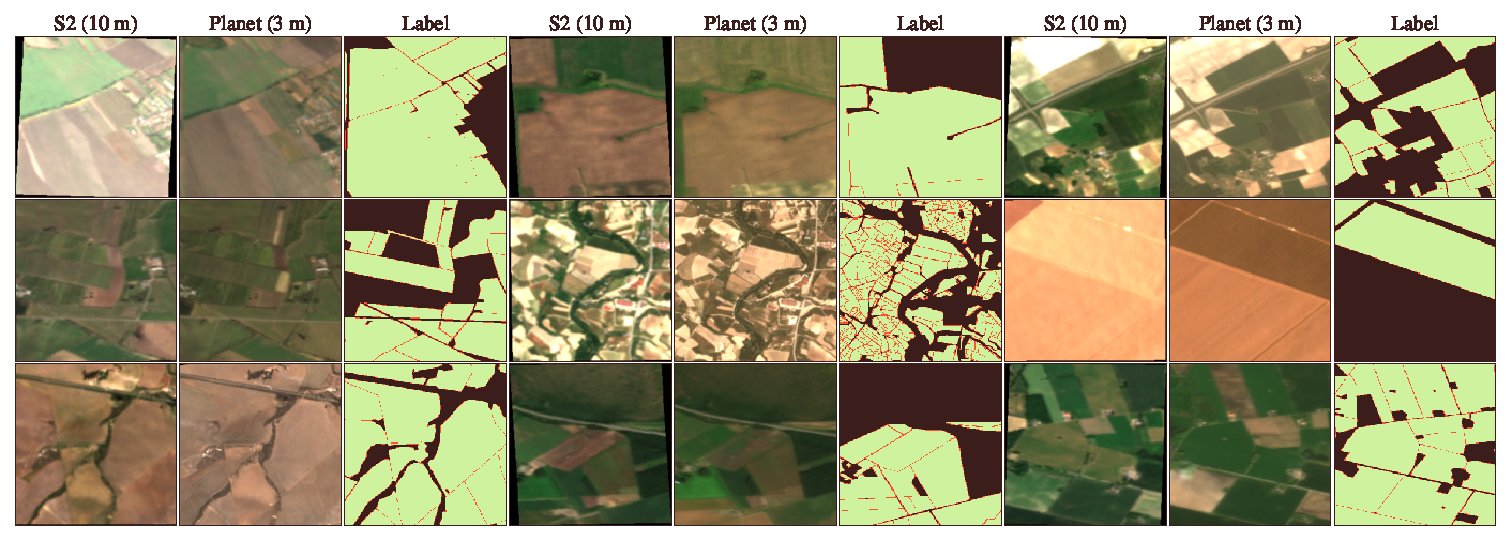
\includegraphics[width=0.95\linewidth]{hero.pdf}
    \captionof{figure}{\textbf{FTW-Planet pairs every Fields of The World patch with co-registered 3\,m PlanetScope imagery and a freshly rasterized 3-class label.} Twelve sample patches spanning the dataset's geographic range. Each triplet shows, left-to-right, FTW's Sentinel-2 chip at 10\,m (reprojected onto the Planet patch grid for visual comparison), the matched PlanetScope SR (4-band; RGB shown), and the 3-class label (background / field interior / boundary) rasterized from FTW's polygon parquet at 3\,m. Reflectance shown is band value $/\,3000$ clipped to $[0,1]$. Boundary class is buffered by 3\,m ($\approx 2$\,px). All samples filtered to UDM2 clear $\geq 99\%$.}
    \label{fig:hero}
\end{center}%
}]
\begin{abstract}
Field-boundary segmentation benchmarks today rely on 10\,m Sentinel-2 imagery, which limits attainable spatial detail and the granularity of the resulting boundary maps.
We release \textbf{FTW-Planet}, a paired companion to the \emph{Fields of The World} (FTW) benchmark in which every FTW Sentinel-2 patch is matched with a co-located 3\,m PlanetScope surface-reflectance image, an 8-band UDM2 quality mask, and a freshly rasterized field-boundary label drawn from FTW's source GeoParquet polygons.
The dataset spans 70{,}484 patches across 25 countries, totals 134{,}267 successfully matched (patch,~window) pairs, and is built from $\sim$6{,}100 unique PSScene COGs accessed via HTTP range reads.
We document the matching pipeline, characterize per-patch quality through UDM2 statistics, and report API-side reliability issues encountered during construction so the community can plan around them.
\end{abstract}

\section{Introduction}

Global field-boundary segmentation underpins yield estimation, irrigation auditing, and parcel-level subsidy verification at country scale.
The \emph{Fields of The World} (FTW) benchmark~\cite{kerner2024ftw} consolidates roughly 1.6\,M parcel polygons across 25 countries on four continents, paired with 10\,m Sentinel-2 imagery in two seasonal windows per patch.
Public benchmarks at finer than 10\,m resolution either cover a single country or pair their imagery with proprietary commercial labels~\cite{tetteh2021ai4smallfarms,wang2022unified,khallaghi2025multitemporal}.
The 10\,m grid limits the smallest field that segmentation models can resolve; smallholder regions in particular suffer~\cite{persello2019delineation,wang2020unified}.

\textbf{We release FTW-Planet}, a paired dataset that brings PlanetScope's $\sim$3\,m, 4-band surface-reflectance imagery~\cite{planetlabs2023psscene} to every FTW patch, alongside the original 8-band UDM2 quality mask and a 3-class label rasterized at the same 3\,m grid.
The dataset is constructed without re-collecting ground truth: we leverage FTW's polygon source files and PlanetScope's COG-based delivery to align imagery and labels per patch.
Our pipeline consists of three phases (search, activate, range-read), is fully resumable, and recovers gracefully from a $\sim$24\% rate of broken signed URLs returned by Planet's activation API.

\textbf{Contributions.}
\begin{itemize}
\itemsep0em
    \item A new paired dataset of 134{,}267 PlanetScope SR + UDM2 + label triples covering 25 countries, all on PlanetScope's native UTM grid at 3\,m.
    \item A scalable Cloud-Optimized GeoTIFF range-read pipeline that bypasses the Orders API and runs on a single HPC node.
    \item Per-patch UDM2 quality statistics for the entire release, plus a re-sampling tool that re-searches alternative scenes when a patch is locally cloudy.
\end{itemize}

\section{Related Work}

\paragraph{Field-boundary benchmarks.}
AI4SmallFarms~\cite{tetteh2021ai4smallfarms} provides 50\,k parcels across South and Southeast Asia at 10\,m. France-ile2018~\cite{wang2020unified} and similar national datasets target single countries.
FTW~\cite{kerner2024ftw} unifies 25 country-scale releases into a single benchmark with a consistent semantic-3-class mask format.
None of these provide commercially-licensed imagery at sub-10\,m resolution that is co-registered with the labels.

\paragraph{High-resolution imagery for parcels.}
Wang et~al.~\cite{wang2022unified} use 3\,m PlanetScope to delineate fields in select French regions but rely on Orders API clipping, which scales poorly. Khallaghi et~al.~\cite{khallaghi2025multitemporal} use Planet Basemaps for multitemporal pixel labeling.
\textbf{We instead access PlanetScope COGs directly via HTTP range reads}, which transfers $\sim$1\,MB per patch out of $\sim$500\,MB scene strips and avoids the Orders queue.

\paragraph{COG access patterns.}
Cloud-Optimized GeoTIFF~\cite{cogspec} enables byte-range reads of just the tiles overlapping a region. STAC~\cite{stacspec} and OGC API---Features expose this pattern in modern catalogs, but the PlanetScope catalog requires asset \emph{activation} before each COG URL becomes available, introducing a thaw step we describe in~\Cref{sec:pipeline}.

\section{Dataset}
\label{sec:dataset}

\subsection{Source data}

\textbf{FTW patches.} Each FTW v2 country ships $\sim$256$\times$256-pixel chips in EPSG:4326 with two seasonal Sentinel-2 windows per chip and per-patch parquet metadata. We use the chip bounding boxes as the AOI for PlanetScope matching (\Cref{tab:scope}).

\textbf{FTW polygons.} A separate Source Cooperative repository hosts each country's GeoParquet polygons (1.6\,M total)~\cite{ftw-source-coop}. We download these directly and rasterize them onto each PlanetScope patch's grid (\Cref{sec:labels}).

\textbf{PlanetScope.} We target the \texttt{ortho\_analytic\_4b\_sr} asset (4-band Surface Reflectance, $\sim$3\,m, uint16 COG) and \texttt{ortho\_udm2} (8-band quality mask, uint8). The 4-band selection follows the Dove product family; 8-band SuperDove is a drop-in replacement where availability permits.

\subsection{Pairing strategy}

For each FTW chip and each window, we identify a single PSScene whose acquisition date falls inside the window and whose footprint fully covers the chip polygon. We rank candidates by date proximity and scene-level cloud cover ($\le$10\%). Patch-level cloud quality is verified \emph{post-hoc} via UDM2 (\Cref{sec:quality}).

\subsection{Pipeline}
\label{sec:pipeline}

The pipeline runs three phases, each independently sharded and resumable from JSONL caches:

\begin{enumerate}
\itemsep0em
    \item \textbf{Search.} Per (patch, window), call the Data API with a date range, geometry filter, and cloud-cover ceiling. Output: best item\_id per patch.
    \item \textbf{Activate.} Deduplicate item\_ids globally; call \texttt{:activate} for SR and UDM2 in parallel. Output: signed Google Cloud Storage URLs.
    \item \textbf{Extract.} Group all (patch, window) by scene, open each COG once with \texttt{rasterio} via \texttt{/vsicurl/}, range-read every member's window, write a local GeoTIFF in PSScene's native UTM at 3\,m. No reprojection.
\end{enumerate}

The activation step dominates wall-time. Cold-storage scenes thaw in 1--46\,min (mean $\sim$200\,s, p99 2{,}763\,s); warm scenes return in 1--5\,s. We saturated Planet's per-account activation queue at $\sim$10/min throughput regardless of client concurrency above 32, which sets a floor on time-to-completion.

\subsection{Labels}
\label{sec:labels}

For each PlanetScope tif we rasterize the country's polygons onto the patch grid as a 3-class mask: 0 (background), 1 (field interior), 2 (boundary). The boundary class is generated by buffering each polygon's exterior ring by 3\,m ($\approx$2 pixels at 3\,m resolution) and rasterizing on top of the interior. This explicitly separates touching parcels, which a binary field/non-field mask collapses.

\subsection{Statistics}

\begin{table}[t]
\centering
\caption{\textbf{Dataset scope.} 25 countries, two seasonal windows per patch. \emph{Success rate} is the fraction of (patch, window) targets with a successfully extracted PlanetScope SR tif.}
\label{tab:scope}
\begin{tabular}{lr}
\toprule
\textbf{Property} & \textbf{Value} \\
\midrule
Countries & 25 \\
Continents & 4 \\
FTW patches & 70{,}484 \\
(Patch, window) targets & 140{,}968 \\
Unique PSScene COGs touched & 6{,}113 \\
Successfully matched pairs & 134{,}267 \\
Success rate & 95.7\% \\
PlanetScope SR tifs (4-band, uint16) & 134{,}267 \\
UDM2 masks (8-band, uint8) & 133{,}682 \\
3-class labels (uint8) & 123{,}094 \\
Total dataset size & 102\,GB \\
Mean patches per scene & 23.0 \\
\bottomrule
\end{tabular}
\end{table}

\Cref{tab:scope} summarizes the release. Patch-to-scene reuse is high ($\sim$23 patches per scene), which makes COG range reads especially efficient: we transfer $\sim$150\,GB of bytes for 102\,GB of materialized patch data, compared to $\sim$3\,TB had we downloaded full strips.

\section{Per-patch quality analysis}
\label{sec:quality}

\Cref{tab:udm2} reports per-patch UDM2 statistics across the full 133\,k UDM2 release, computed by reading the patch-area windows directly from each mask and counting positive pixels per band. \textbf{86.6\%} of patches are usable at a strict threshold (clear$\,\ge\,$95\%, unusable$\,\le\,$5\%).

\begin{table}[t]
\centering
\caption{\textbf{Per-patch UDM2 statistics.} Fractions are pixel-area within the patch. Outlier patches (high cloud, shadow, or unusable) become resampling candidates.}
\label{tab:udm2}
\begin{tabular}{lcccc}
\toprule
Band & median & p90 & p99 & max \\
\midrule
clear & 100\% & 100\% & 100\% & 100\% \\
cloud & 0\% & 0\% & 88\% & 100\% \\
shadow & 0\% & 0\% & 21\% & 100\% \\
light haze & 0\% & 0\% & 41\% & 100\% \\
unusable & 0\% & 0.8\% & 51.9\% & 100\% \\
\bottomrule
\end{tabular}
\end{table}

\paragraph{Patch-level resampling.}
The original search filter rejects scenes whose \emph{scene-level} cloud cover exceeds 10\%; this is a coarse proxy because clouds can concentrate over a single patch even in a low-cloud scene. We provide a re-sampling tool that, for each patch failing any per-band threshold, searches alternative scenes within the same season ($\pm$60\,d), probes their UDM2 over the patch AOI, and replaces the SR + UDM2 pair when a candidate strictly improves quality. The tool re-uses the same activation cache and runs in $\sim$5--8\,h for the full release.

\paragraph{Per-country variation.} The cloudiest countries by % usable are Portugal (40.9\%), South Africa (56.5\%), and the Netherlands (76.5\%); Brazil and Croatia exceed 98\%. Smallholder regions (e.g., India) have low \emph{coverage} per patch ($\sim$1\% field pixels) but high clear-sky fractions.

\section{Operational notes}

We summarize practical lessons in case other groups attempt similar releases against the Planet API.

\paragraph{Activation reliability.} Across 6{,}113 unique scenes, $\sim$24\% of \texttt{:activate} calls returned URLs that subsequently failed with HTTP 400 on the first range read. A second \texttt{:activate} call typically returned a different, working URL; reactivating the failed item\_ids recovered 99\% of these patches. Our final pipeline includes an automatic reactivation pass.

\paragraph{Throughput.} Cold-storage thaw, not bandwidth, is the bottleneck. Activation throughput plateaus around 10\,scenes/min per account; total dataset construction took $\sim$17\,h end-to-end on a single HPC node, dominated by activation. Pre-warming a list of scene IDs would compress this substantially.

\paragraph{Cost-effective access.} For windowed access patterns, COG range reads via \texttt{/vsicurl/} are $\sim$100$\times$ faster than Orders API clipping and require only the Data API role. Documenting this access pattern more prominently would lower the barrier for other dataset projects.

\section{Benchmark}
\label{sec:benchmark}

We train and evaluate field-boundary segmentation models on FTW-Planet to
characterize the dataset and to compare against the FTW Sentinel-2
baseline. To ensure a fair held-out comparison we adopt the FTW
\textbf{CC-BY split}~\cite{kerner2024ftw}: 14 countries are used for
training (austria, brazil, corsica, denmark, estonia, finland, france,
india, luxembourg, netherlands, rwanda, slovakia, spain, vietnam) and
the remaining 11 are entirely held out at test time (belgium, cambodia,
croatia, germany, kenya, latvia, lithuania, portugal, slovenia,
south africa, sweden). All metrics in this section are macro-averaged
per country following the FTW protocol.

\paragraph{Recipe.} We follow the PRUE recipe~\cite{kerner2024ftw}:
EfficientNet--UNet, in\_channels$\,=\,$8 (window B then A, 4 bands each),
3-class output, \texttt{logcoshdice} loss with class weights
$[0.05, 0.20, 0.75]$, ignore index 3 (padded regions), 100 epochs of
AdamW @ $10^{-3}$, batch size 32 (B7: 8) at random 512$\times$512
crops, bf16-mixed, kornia GPU augmentations (90$^\circ$ rotations and
H/V flips). All inputs are scaled by $/10000$. Inference pads each
patch to at least $512\times512$ (matching the training crop) before a
single forward pass; we previously verified this rule is worth +24\,pts
pixel IoU over padding to the nearest multiple of 32.

\paragraph{Auxiliary heads.} We ablate two auxiliary regression heads
attached to the final UNet decoder feature map (16~channels at full
resolution): (i)~an \textbf{SDF head} predicting the clipped Euclidean
distance to the nearest field boundary, supervised with $L_1$ against a
target computed at data-loading time and trained jointly with the seg
loss at weight $0.2$; and (ii)~a \textbf{frame field head} predicting a
4-PolyVector field $f(z)\,=\,z^4 + c_2 z^2 + c_0$ whose four roots
encode the local boundary tangent directions~\cite{girard2021ffl}.
Frame-field supervision uses the GT boundary tangent (rotated Sobel
gradient of the field-interior mask) via the alignment loss
$|f(\tau)|^2$, plus an $L_2$ spatial smoothness term on $(c_0, c_2)$.

\paragraph{Post-processing.} For instance separation we use
marker-controlled watershed: seeds from $h$-maxima on the topographic
surface, basins flooded inside the predicted field mask. With an SDF
head the topographic surface is the predicted SDF directly; without it
we use the Euclidean distance transform of the predicted boundary.

\paragraph{Results.} Table~\ref{tab:heldout} reports macro-averaged
metrics on the 11 held-out countries (and on the 9-country subset that
excludes kenya, presence-only, and portugal, where every model
collapses to $\le 0.10$ pixel IoU). The S2 CC-BY checkpoint
from~\cite{kerner2024ftw} is the only fully apples-to-apples baseline;
S2 PRUE-B7 is trained on the full 25-country set and would constitute
an unfair comparison on these held-out splits.

\begin{table}[t]
    \centering
    \small
    \caption{Held-out benchmark. All models trained on the FTW CC-BY
    14-country split and macro-averaged over either all 11 held-out
    countries or the 9 that retain non-trivial field coverage and
    polygon labels.}
    \label{tab:heldout}
    \begin{tabular}{lcccc}
\toprule
Model & Pix IoU & Pix Prec & Pix Rec & Obj F1 \\
\midrule
\multicolumn{5}{l}{\textit{9 (excl K+P) held-out countries (macro avg)}}\\
S2 CCBY (B3, CE) \cite{kerner2024ftw} & \textbf{0.608} & \textbf{0.834} & 0.706 & 0.317 \\
FTW-Planet B3 (PRUE recipe) & 0.541 & 0.815 & 0.637 & 0.323 \\
FTW-Planet B3 + SDF aux & 0.520 & 0.814 & 0.616 & 0.320 \\
FTW-Planet B3 + frame-field aux & 0.542 & 0.825 & 0.632 & 0.302 \\
FTW-Planet B7 + SDF aux & 0.571 & 0.785 & \textbf{0.709} & \textbf{0.334} \\
\midrule
\multicolumn{5}{l}{\textit{all 11 held-out countries (macro avg)}}\\
S2 CCBY (B3, CE) \cite{kerner2024ftw} & \textbf{0.537} & \textbf{0.828} & 0.619 & 0.262 \\
FTW-Planet B3 (PRUE recipe) & 0.444 & 0.750 & 0.570 & 0.265 \\
FTW-Planet B3 + SDF aux & 0.478 & 0.734 & 0.623 & \textbf{0.279} \\
FTW-Planet B3 + frame-field aux & 0.446 & 0.700 & 0.574 & 0.249 \\
FTW-Planet B7 + SDF aux & 0.468 & 0.642 & \textbf{0.641} & 0.274 \\
\bottomrule
\end{tabular}

\end{table}

Three takeaways:
\begin{itemize}
\itemsep0em
\item On pixel IoU, S2 CC-BY narrowly leads our best FTW-Planet
configuration (0.608 vs 0.571 on the 9-country subset).
PlanetScope's 3$\times$ GSD advantage does \emph{not} translate to
better pixel-level field IoU once the segmentation must generalize to
held-out countries; the Sentinel-2 model trained on the same 14
countries transfers better.
\item On \emph{object-level} F1, our FTW-Planet B7+SDF model leads
(0.334 vs 0.317), suggesting that higher-resolution imagery improves
field \emph{instance} separation even when pixel-level accuracy lags
slightly. This is the metric most relevant for downstream
polygonization.
\item The SDF auxiliary head improves held-out robustness on hard
transfer cases. In particular, on portugal (low field coverage,
unfamiliar terraced landscape) the B3 baseline drops to 0.007 pixel
IoU; adding the SDF head recovers it to 0.576. The frame-field head
does not improve held-out accuracy in our configuration; further
sweep of loss weights is required.
\end{itemize}

\begin{table}[t]
    \centering
    \scriptsize
    \caption{Per-country pixel IoU on the 11 held-out countries:
    S2 CC-BY (B3) vs our best FTW-Planet (B7 + SDF). Both models trained
    on identical 14 CC-BY countries.}
    \label{tab:heldout_pc}
    \begin{tabular}{lcccc}
\toprule
Country & S2 CCBY IoU & Planet B7+SDF IoU & $\Delta$ IoU & Planet Obj F1 \\
\midrule
belgium & 0.599 & \textbf{0.625} & +0.026 & 0.501 \\
cambodia & \textbf{0.383} & 0.357 & -0.026 & 0.041 \\
croatia & 0.518 & \textbf{0.607} & +0.088 & 0.334 \\
germany & \textbf{0.739} & 0.327 & -0.412 & 0.121 \\
kenya & \textbf{0.392} & 0.006 & -0.385 & 0.003 \\
latvia & \textbf{0.753} & 0.652 & -0.101 & 0.438 \\
lithuania & 0.554 & \textbf{0.631} & +0.077 & 0.443 \\
portugal & \textbf{0.041} & 0.000 & -0.041 & 0.000 \\
slovenia & 0.430 & \textbf{0.513} & +0.082 & 0.262 \\
south africa & \textbf{0.758} & 0.638 & -0.120 & 0.312 \\
sweden & 0.740 & \textbf{0.789} & +0.048 & 0.555 \\
\midrule
Macro (9, excl K+P) & 0.608 & 0.571 & -0.037 & 0.334 \\
\bottomrule
\end{tabular}

\end{table}



\textbf{Coverage.} 5{,}715 (4.1\%) of (patch, window) targets have a chosen scene that never produced a usable URL despite repeated reactivation; 343 (0.2\%) hit hard Planet-side asset failures. These patches retain their FTW Sentinel-2 imagery but have no PlanetScope companion in this release.

\textbf{Temporal misalignment.} The PlanetScope acquisition date is the closest cloud-free match to the FTW season midpoint, not the exact S2 acquisition date. Differences are typically $<$2\,weeks but can exceed a month in cloudy regions.

\textbf{Future work.} (i)~Add 8-band SuperDove samples where available for the same patches. (ii)~Provide pre-computed augmented mosaics across both seasonal windows. (iii)~Close the held-out pixel-IoU gap to Sentinel-2: candidate directions include longer pre-training, multi-temporal stacks beyond the two FTW windows, and instance-aware decoders (e.g.\ a polygon head conditioned on the frame field).

\section{Conclusion}

FTW-Planet is a 3\,m PlanetScope companion to the Fields of The World benchmark, complete with co-registered 3-class field-boundary labels and per-patch UDM2 quality statistics. The construction pipeline---a search/activate/range-read three-phase chain---runs on a single HPC node and is fully resumable. We hope the release lowers the barrier to high-resolution field-boundary research and that the operational notes help other groups avoid the API-reliability pitfalls we encountered.

\bibliographystyle{ieeenat_fullname}
\bibliography{refs}

\end{document}
